\documentclass{itecreport-zh}

\title{硬件课程设计实验报告}{Course Exercise of Hardware Design Report}
\author
{贾镇远}
{Zhenyuan Jia}
\supervisor
{黑晓军\hspace{1em}副教授}
{Ass. Prof. Xiaojun Hei}
\date{2017}{7}{5}

\zhabstract{
	这是一个硬件课程设计实验报告。
	该硬件课程设计由 \emph{Client} 小组完成,小组成员:


	贾镇远、肖法鲁、万政

}
\zhkeywords{硬件课程设计,实验报告}

\enabstract
{
    This is a report of a hardware course design report.
    The deisgn is compeleted by the \emph{Client} group, which is made up of

    
    Zhenyuan Jia, Zheng Wan and Falu Xiao.
}
\enkeywords
{Hardware Course Design, Report}

\begin{document}

\frontmatter
\maketitle
\makeabstract
\tableofcontents
% \listoffigures
% \listoftables
\mainmatter

\chapter{引言}\label{chapter:1}
\section{编写目的}\label{sec:1}
华中科技大学电信学院2014级于本学期开设硬件课程设计课程。本报告为智能路由器选题下Client小组为本次课程设计撰写的最终实验报告。
\section{背景}
华科校园网使用的是锐捷的网络认证管理方案。因此,学生使用校园网必须进行锐捷认证,而且一个校园网帐号在同一时间只允许一台设备登录校园网。这样在使用时十分不方便,而且也不能多设备同时使用上校园网。于是我们想开发一个代理设备,对校园网进行代理认证,不仅省去了每次都要登录上网的麻烦,还能多设备同时上网。
\section{课题调查}
学校的锐捷认证有两种方式:
\begin{enumerate}
    \item 802.1x认证
    \item Web认证
\end{enumerate}

如下图:

\begin{figure}[!h]
\centering
  \begin{subfigure}[b]{0.3\textwidth}
  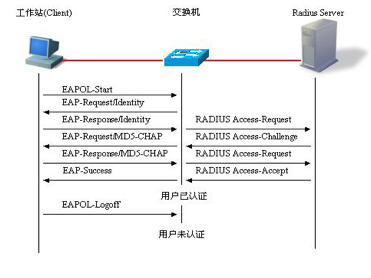
\includegraphics[width=\textwidth]{8021x.png}
  \caption{802.1x认证}
  \end{subfigure}
  ~
  \begin{subfigure}[b]{0.3\textwidth}
  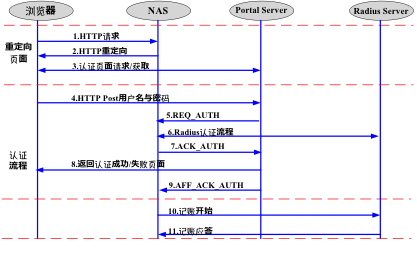
\includegraphics[width=\textwidth]{web.png}
  \caption{Web认证}
  \end{subfigure}
\end{figure}

其中802.1x集中认证是通过认证客户端向认证交换机申请认证,交换机将认证信息提交给中心认证服务器,服务器调取数据库确认认证信息的真伪,再将信息发给交换机,由交换机实际控制客户端的网络连接状态。

而Web集中认证则是增加了一个Potal服务器,提供HTTP服务,用户在WEB页面上进行认证,认证信息由Potal服务器提交给中心认证服务器,但是用户的网络连接控制还是由交换机来实现。


MentoHUST是一个支持Windows、Linux、Mac OS下的第三方锐捷认证的程序(附带支持赛尔认证)。它支持华科的锐捷认证,它是开源的项目,我们选用MentoHUST作为认证软件。


OpenWrt是适合于嵌入式设备的一个Linux发行版。相对原厂固件而言,OpenWrt不是一个单一、静态的固件,而是提供了一个可添加软件包的可写的文件系统。这使用户可以自由的选择应用程序和配置,而不必受设备提供商的限制,并且可以使用一些适合某方面应用的软件包来定制你的设备。对于开发者来说,OpenWrt是一个框架,开发者不必麻烦的构建整个固件就能得到想要的应用程序;对于用户来说,这意味着完全定制的能力,与以往不同的方式使用设备,OPKG包含超过3500个软件。

\chapter{实际开发结果}

\section{产品}
\begin{figure}[!h]
\centering
  \begin{subfigure}[b]{0.4\textwidth}
  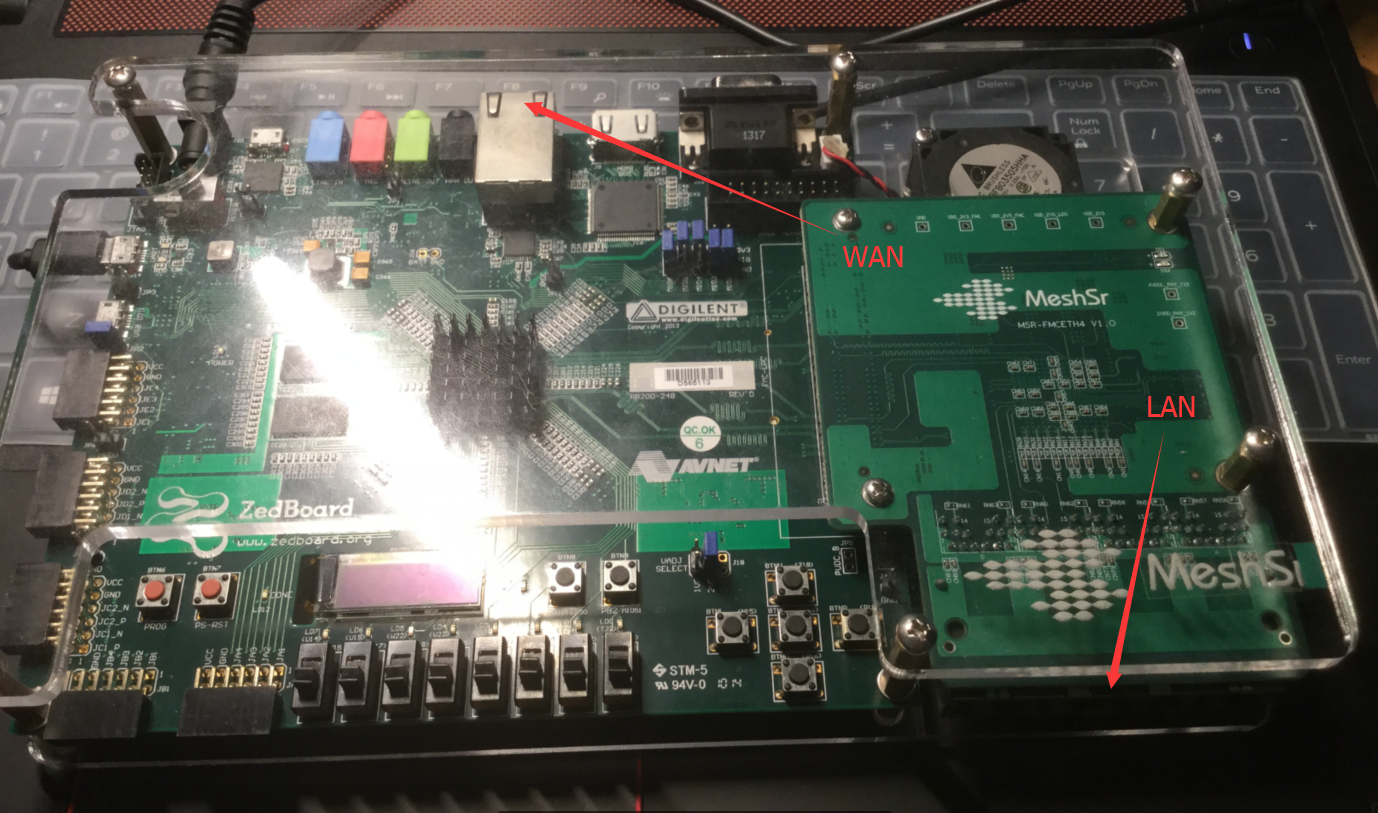
\includegraphics[width=\textwidth]{product.png}
  \caption{实物图}
  \end{subfigure}
~
  \begin{subfigure}[b]{0.4\textwidth}
  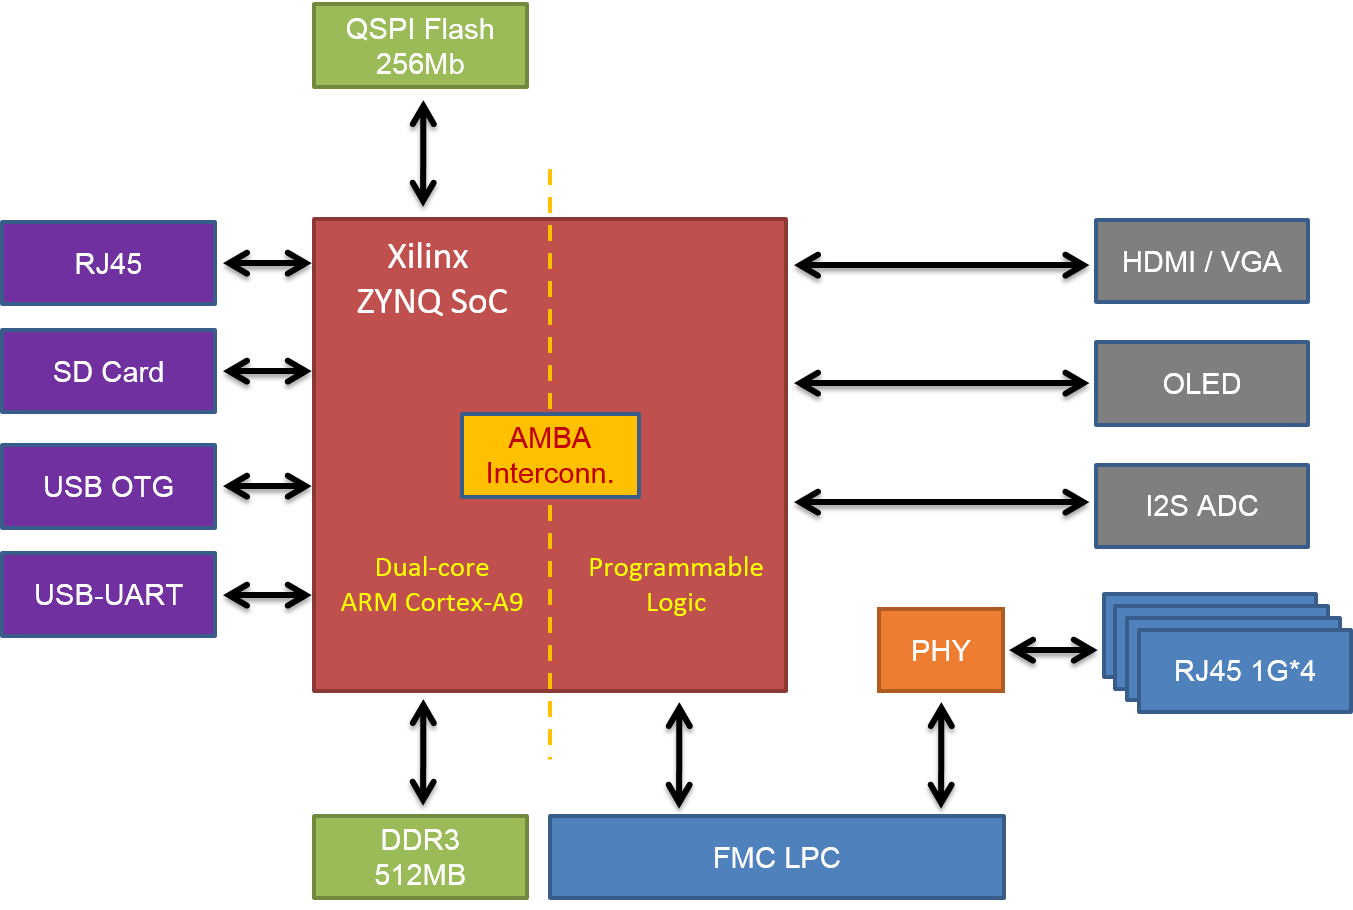
\includegraphics[width=\textwidth]{ons20-hw.png}
  \caption{结构}
  \end{subfigure}
\end{figure}
我们使用的是老师提供的ONetSwitch20开发板。该开发板母板是一块Xilinx公司的Zedboard开发板,然后通过FMC接口扩展了一块带有四个GE口的扩展板。

\begin{figure}[!h]
\centering
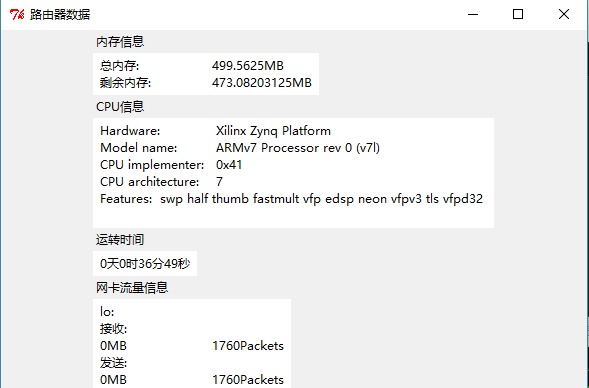
\includegraphics[width=.8\textwidth]{zynqinfo.png}
\caption{远程监视}
\end{figure}

\begin{figure}[!h]
\centering
  \begin{subfigure}[b]{0.5\textwidth}
  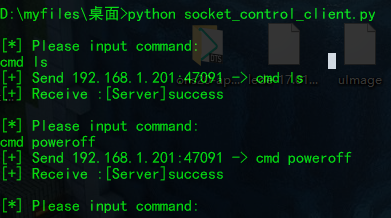
\includegraphics[width=\textwidth]{zynqctrl1.png}
  \caption{远程控制客户端}
  \end{subfigure}
  ~
  \begin{subfigure}[b]{0.4\textwidth}
  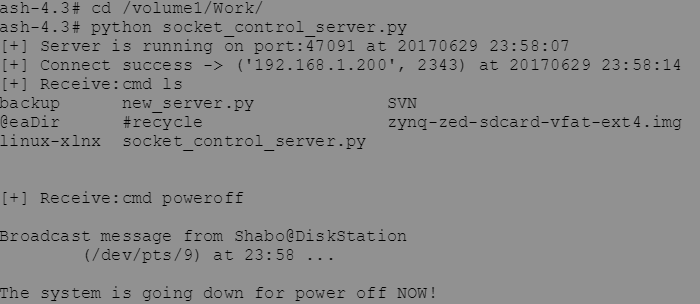
\includegraphics[width=\textwidth]{zynqctrl2.png}
  \caption{远程控制服务端}
  \end{subfigure}
\end{figure}

linux设备远程监控程序。可以根据linux设备的IP与设备通信,从而获取设备的信息或对设备进行控制。

\section{主要功能和性能}

\begin{enumerate}
    \item 校园网锐捷认证
    \item 基本的家庭网关功能
    \item 通过网络远程监控
\end{enumerate}

\begin{figure}[!h]
\centering
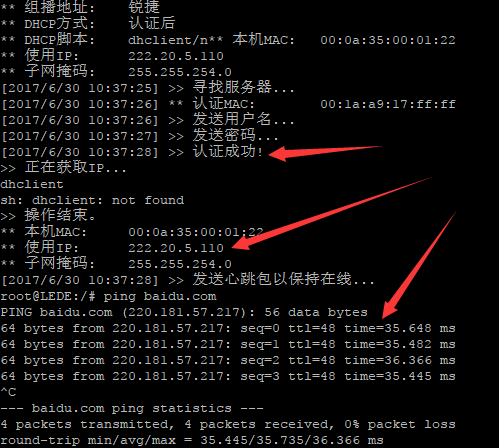
\includegraphics[width=.6\textwidth]{ruijie.png}
\caption{锐捷认证结果}
\end{figure}

开发板使用MentoHUST开源软件,能通过校园网锐捷认证,进行上网,上图认证成功并且与百度主页ping通。


母板的GE口作为wan口连上校园网,扩展版上的四个GE口作为lan口,连接内网设备。用MentoHUST锐捷认证程序在wan口进行校园网认证,电脑等终端设备接在lan口上,便可以通过开发板上网。


开发板连上网络获取IP地址之后,开启服务端程序。可以通过IP地址连接上开发板并与之通信,获取开发板的CPU负载、内存占用率、磁盘使用情况、运行时间、网络情况等数据。

\section{开发过程}
\begin{enumerate}
    \item 将OpenWRT系统刷入Zybo开发板


    我们刚开始是只有Zybo的开发板作为硬件课设的实验平台。我们发现OpenWRT项目官方对Xilinx的几块板子有支持,其中就有Zybo,于是我们将源码下载下来写入存储卡,系统成功运行。

    \item 校园网锐捷认证


    然后搭建交叉编译环境,将交叉编译出适配的MentoHUST可执行程序放入开发板,程序成功运行,并进行了锐捷认证。

    \item 将前期的工作移植到ONetSwitch20开发板上


    这里我们换了开发平台,用了叠锶公司的开源硬件平台ONetSwitch20。这个开发板母板是Xilinx的Zedborad,OpenWRT也是支持的,先将OpenWRT烧入存储卡,交叉编译,成功认证。

    \item 驱动四个扩展以太网口


    开发板扩展板有四个扩展以太网口,于是自然是要把几个以太网口驱动起来,做成多网口设备。发现官方提供了开发板的交换机例程,于是选用叠锶的BOOT.BIN、设备树文件和内核,用了LEDE的文件系统。开发板成功启动,四个以太网口也成功驱动。LEDE是成熟的特意为网络设备开发的发行版,这里可以将开发板直接配置成家庭网关。将剩下几个网口配置上IP地址,然后发现没法网络访问了,意识到是VLAN的问题————这里开发板在我的寝室内网环境下,开发板网口与内网IP段冲突了,开发板不知道包往哪个网口发送。到LEDE的网页配置,发现不支持VLAN,应该是内核没有开启802.1q支持。

    \item 重新配置编译内核,支持VLAN和NAT


    于是重新配置编译Linux内核,叠锶提供了适配的Linux源码。成功开启并配置VLAN,但是内外网是不通的。用iptables设置转发规则,发现内核不支持。再次重新编译,好在已经熟了。果然成功开启,现在基本已经是一个可用的家庭网关了。

    \item 编写远程监控程序


    我们考虑到,基础的功能虽然花费了时间精力,但是展示起来效果不太好,因为做成了基本的网关,就是连上校园网,连上设备,然后设备能通过开发板上网,没有一些amazing的效果,于是我们打算做一些应用型的功能在上面。我们想到了几套应用。
      \begin{enumerate}
        \item 一个网络摄像头的开源项目,开发板通过USB连上开发板,开发板同时通过网页将视频流送出
        \item 写一个程序,获取开发板的信息或者控制,并通过Socket通信
      \end{enumerate}
      这些想法都是很有实用价值的。但是在后面实践中,发现开发板的USB接口没法用,在固件层就没有进行连接,更改硬件工程,对USB进行驱动,剩余的时间难以完成,我们选择第二个,比较偏应用层,基本没有问题。
\end{enumerate}
\section{部分代码}
硬件课设很多是固件层和操作系统的工作,这里展示锐捷认证和远程监控的部分代码。


MentoHUST代码
\chapter{开发工作评价}
\section{对生产效率的评价}
\section{对产品质量的评价}
\section{对技术方法的评价}
\chapter{经验与教训}


\end{document}


